% vim: set ft=tex foldlevel=2 spelllang=en:
\cleardoublepage

% TODO: Shouldn't this be "Final remarks" or so?
\chapter{Final Remarks}
% \minitoc

\section{Achieved Goals}

We consider that the main goals set at the beginning of this project
(\autoref{sec:project-goals}) have been fullfilled. In particular:

\begin{itemize}

	\item Developing an automatic binding system for the Lua programming
	language, allowing seamless usage of C libraries.

	\item Using the DWARF debugging information contained in ELF shared object
	files to pinpoint the details about function, and involved data types.

	\item Converting data values transparently between Lua and C.

	\item Providing a reference implementation for GNU/Linux running on the
	x86\_86 architecture.

	\item Avoiding modifications of the internals of the Lua VM. The
	implementation was achieved using exclusively the Lua C API.

\end{itemize}

The C programming language was used to develop \Eol*, a Lua module which
implements a FFI for Lua using the DWARF debugging information to gain
knowledge about the types and functions available in ELF shared object files.
Separating the code which deals with native function invocation allows
selecting which method is used to invoke native functions from Lua at
build-time. Two backends were implemented: one using \verb|libffi|, and
a second one using JIT compilation (by means of DynASM) for the Intel x86\_64
architecture to generate the needed glue code.

Additionally, a test harness for Lua has been developed, due to the existing
Lua unit testing frameworks aborting their execution in the event of a crash
of the process. The harness has been implemented mostly in Lua, plus a small
helper module written in C to access Unix system calls which are not covered
by the Lua standard library.

The implementation of \Eol* consists of approximately 7.000\todo{Update
numbers later if needed} lines of code (standard LOC, ignoring comments, see
\autoref{fig:eol-loc}), of which the biggest part is the implementation of the
\Eol* Lua module, as expected.

\begin{figure}[ht]
	\centering
	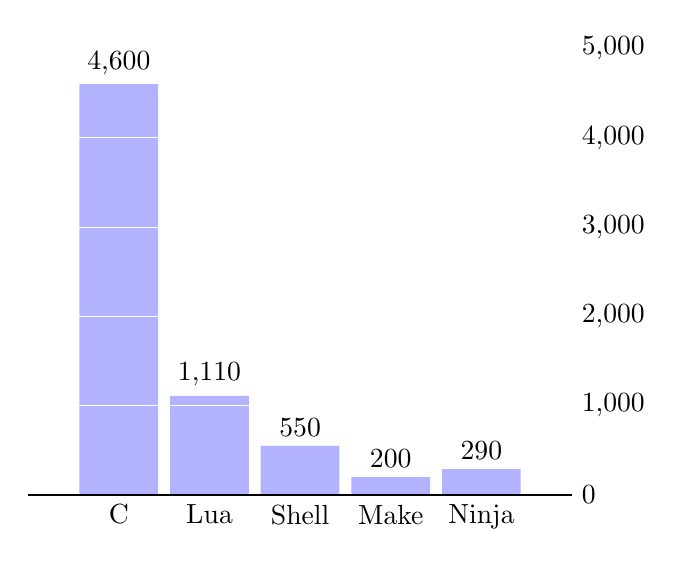
\begin{tikzpicture}
		\begin{axis}[
			style={/pgf/number format/assume math mode=true},
			width=0.7\textwidth,
			ybar, axis on top,
			ymajorgrids, tick align=inside,
			major grid style={draw=white},
			enlarge y limits={value=.1,upper},
			axis x line*=bottom,
			axis y line*=right,
			y axis line style={opacity=0},
			enlarge x limits=0.25,
			tickwidth=0pt,
			xtick=data,
			bar width=1cm,
			symbolic x coords={C, Lua, Shell, Make, Ninja},
			nodes near coords,
			ymin=0,
			]
			\addplot[draw=none, fill=blue!30] coordinates {
				(Lua,1110) (C,4600) (Shell,550) (Make,200) (Ninja,290)
			};
		\end{axis}
	\end{tikzpicture}
	\caption{Lines of code in \Eol*, per language.}
	\label{fig:eol-loc}
\end{figure}

Last but not least, the \Eol* FFI module has been tested thoroughly, in two
ways:

\begin{itemize}

	\item With an automated test suite, which can be used for regression
	testing—and has been used as such to ensure that the behaviour of code
	generated by the JIT compilation of function invocations works the same
	way as the \verb|libffi|-based method.

	\item Writing example programs which exercise the module. These use third
	party libraries used in real world projects, so the example programs
	stress the FFI in the way it is intended to be used.

\end{itemize}



\section{Lessons Learned}

During the development of the project, the specification of the ELF and DWARF
standards has been analyzed, and the relevant parts which are useful for
implementing a \gls{FFI} have been identified. A comprehensive understanding
of the specification was acquired thanks to the following documentation:

\begin{itemize}

	\item \emph{How Debugging Works}~\cite{howdebugworks}: Tutorial-style
	series of articles which give a good overall overview of how debugging
	information is embeeded into compiled object code.

	\item \emph{System V Application Binary Interface Edition
	4.1}\cite{elfspec-sysv}: Contains the original (non normative)
	  specification of the ELF object file format. Though newer, normative
	  versions of the specification exist, this version explains the concepts
	  needed to understand the DWARF debugging information in an more
	  approachable way.

	\item \emph{DWARF Debugging Information Format Version
	4}~\cite{dwarfspecv4}: Normative specification of the DWARF debugging
	  information format.

\end{itemize}

Existing FFI implementations for Lua have been analyzed to understand how they
work, which was a valuable knowledge to keep in mind while designing how \Eol*
bridges native code to Lua. In particular, the LuaJIT \verb|ffi| module was
taken as a prime example of a proven solution which is popular in the Lua
community. The following documents were instrumental for the design of the
developed solution:

\begin{itemize}

	\item \emph{FFI semantics}~\cite{lj-ffi-semantic}: Describes how the
	module interacts both with Lua, and the compiled C code.

	\item \emph{ffi.* API functions}~\cite{lj-ffi-api}: Describes the API
	of the \verb|ffi| module.

\end{itemize}

Implementing the JIT code generation required learning how to use LuaJIT's
DynASM, which lacks official documentation. It was also needed to learn to
program in assembler for the Intel x86 platform, and its \gls{ABI} calling
conventions during the development of the JIT code generator.


\section{Future Directions}

Every software project has room for improvement and continued refinement, and
\Eol* is no exception. There are a number of features which have been
knowingly left out of the present project, in order to keep its scope under
control. It is the intention of the author to keep developing \Eol* as a Free
Software project, and there are a number of ideas for future development which
have surfaced during the realization of its current version.

The following are ideas which are complex to realize, and even though working
on them would require a big development effort, they open the path to exciting
new possibilities:

\begin{itemize}

	\item Defining an on-disk format for type and function information. The
	idea would be to obtain the information from the DWARF debugging
	information, and store it in a format which is optimized for faster
	reading. The files in this new format would be used for on-disk caching.

	\item Using the file format implemented from the previous bullet point,
	allow reading type information directly from it, without requiring that
	the ELF shared objects include DWARF debugging information.

	\item Saving the generated code to disk in ELF object files, when \Eol* is
	built with JIT code generation enabled.	The generated code could be loaded
	reusing the Lua module loader.

	\item Implementing support for reading debugging information in formats
	other than DWARF. Ideally, there would be an interface that a “type
	information provider” component could implement, and the DWARF provider
	would be just one of many.

\end{itemize}

The following fall into the category of improvements which can be done with
a moderate effort, and would certainly provide added value to the project:

\begin{itemize}

	\item Building a community around \Eol* is already Free Software, it lacks
	a community, and it would be interesting to foster a healthy community
	around the project. That would require writing more documentation (e.g.
	a quick start tutorial, a walkthough of the features), and having public
	communication channels (e.g. a mailing list, an \gls{IRC} chat room,
	participating in the \verb|lua-l| list...).

	\item Ensuring the compatibility of \Eol* works Lua 5.2, and 5.1. Those
	are the versions more widely deployed\todo{See if it's possible to add
	a citation}.

	\item Enabling use of \Eol* with LuaJIT. Most modules using the Lua C API
	can be built for LuaJIT as well. LuaJIT is designed to be compatible with
	Lua	5.1, while the current Implementation targets version 5.3.

	\item Implementing JIT compilation of function invocations for
	architectures other than x86, and x86\_64. This can be done with ease for
	the other architectures supported by DynASM: ARM, MIPS, and PowerPC.

\end{itemize}


\section{Post-Mortem Analysis}

